\documentclass[a4paper,11pt]{scrartcl}

\usepackage[ngerman]{babel} 
\usepackage[T1]{fontenc}
\usepackage[utf8]{inputenc}
\usepackage{hyperref}

\usepackage{amsmath,amsfonts,amssymb}
\usepackage{graphicx}
\usepackage{siunitx}

\usepackage{epstopdf}

\setcounter{section}{3}


\begin{document}
\hfill Alexander Schnapp

\hfill Max Menges

\begin{center}
\underline{\Huge{Intro HPC: Blatt 3}}\\
\large{04.11.1014}\\
\end{center}


\subsection{Moores Law}
Nach \emph{Moores Law} verdoppelt sich die Prozessorleistung alle 18 Monate. Für die Rechneleistung $R$ gilt dann nach $a$ Jahren bei momentaner Leistung vom $R_{peak}$\footnote{\url{http://top500.org/lists/2014/06/}}:

\begin{align*}
R&=R_{peak}\cdot 2^{\frac{a}{1.5}} \Rightarrow a = 1.5\cdot \log_2{\frac{R}{R_{peak}}}
\end{align*}

Damit wird ein Exaflop nach \emph{Moores Law} in 6.28 Jahren erreicht.
\begin{align*}
1.5\cdot \log_2{\frac{1000}{54.9}}&=6.28
\end{align*}

Mit den Werten der TOP500 Liste jeweils aus dem November 2007 und 2011 ergibt sich:
\begin{align*}
    a&= \frac{4}{\log_2{\frac{R_{2011}}{R_{2007}}}}=0.94
\end{align*}

Also ein Vedopplung alle 11.3 Monate statt alle 18 Monate wie von Moore vorhergesagt. Damit wir auch ein Exaflop früher erreicht, und zwar in 3.9 Jahren.\\

\subsection{Amdahls Law}
\paragraph*{b)}Verbessert man die Wurzelberechnung um einen Faktor von 10 benötigt man noch ($20/10+80=82$) $82\%$ der zuvor benötigten Zeit. Im Falle der Verbesserung der generellen FP Rechnungen kommt man auf $50+50/1,6=81,25$. Man Braucht also mit etwa $81\%$ knapp weniger Zeit.
\paragraph*{c)}
Es gilt Amdahls Law:
\[
Speedup=\frac{1}{(1-P)+P/N}
\] 
Löst man dieses nach $P$ auf und setzt $N=128$ und den gewünschten Speedup von 100 ein so kommt man auf
\[
P=\frac{\frac{1}{Speedup}-1}{1/N-1}=0.9978
\]
und damit auf einen maximalen seriellen Anteil von 0,22\%.
\subsection{Measure Latency}

Der Quelltext liegt unter \verb+../3/3_3/pingpong.cpp+. Makefile zum Compilieren und ausführen liegt bei. \\

Es werden pro Nachrichtengröße jeweils 8 Nachrichten geschickt (mehr hat MPI irgendwie nicht erlaubt). Das Pingpong Programm wurde zwei mal ausgeführt, einmal mit beiden Prozessen auf einer Maschine ("`Cache"' im plot) sodass der Nachrichtenaustausch via \emph{Cache} oder Hauptspeicher erfolgt. Beim zweiten Mal Ausführen würden beide Prozesse auf unterschiedlichen Rechnern (\verb+creek04+, \verb+creek06+) ausgeführt. Die Nachrichten müssen also einmal über das Netzwerk ("`Ethernet"' im plot).\\

\begin{figure}[!ht]
\centering
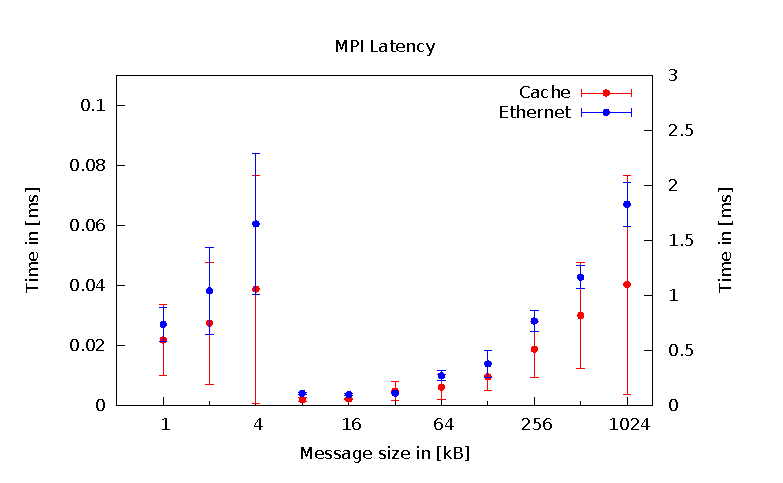
\includegraphics[width=0.7\textwidth,keepaspectratio]{3_3/data/plot.eps}
\end{figure}

Dabei fallen drei sachen auf: 

\begin{itemize}
    \item Ethernet ist $\approx 10$ mal langsamer als der Nachrichtenaustausch auf einem Rechner.
    \item Die relativen Fehler der Durchschnittslatenz ist bei Ethernet deutlich kleiner. Ethernet ist zwar langsam aber stabil.
    \item Die Latenz nimmt bei einer nachrichtengröße von $8kB$ deutlich ab. Vermutlich puffert MPI ausgehende Nachrichten und verschickt diese erst wenn der Puffer voll ist (oder nach gewisser Zeit). Das sorgt für hohe Latenz bei kleinen Nachrichten. Da die Latenz bei $8kB$ wieder fällt scheint der Puffer zwischen 4 und 8 $kB$ groß zu sein.
\end{itemize}





\subsection{Measure Bandwidth}

\end{document}
